\documentclass{article}
\usepackage[none]{hyphenat}
\usepackage{graphicx}
\usepackage[]{algorithm2e}
\usepackage{program}
\usepackage{eufrak}
\usepackage[a4paper, total={6in, 8in}]{geometry}
\graphicspath{ {images/} }
\begin{document}
	
	\title{Bootstrap Estimation of a Non-Parametric Information Divergence Measure}
	\author { Prad Kadambi and Visar Berisha \\
		\small Arizona State University \\
		\small Department of Electrical, Computer and Energy Engineering}
	\date{}
	\maketitle
	
	%----------------------------------------------------------------------------
	\begin{abstract}
		
		This work details the bootstrap estimation of a nonparametric information divergence measure, the $D_p$ divergence measure, applied to the binary classification problem.\ To address the challenge posed by computing accurate divergence estimates given finite size data, a bootstrap approach is used to in conjunction with a power law curve to calculate an asymptotic estimate of the divergence measure in question. Monte Carlo estimates of $D_p$ are found for increasing values of sample data size, and a power law fit is used to find the asymptotic convergence value of the divergence measure as a function of sample size.\ The fit is also used to generate a confidence interval for the estimate which allows us to characterize the quality of the estimator.\ The results obtained for the divergence measure are then compared to several other resampling methods.\  Utilizing the inherent relation between divergence measures and classification error rate, an analysis of the Bayes Error Rate of several test data sets is conducted via the power law estimation approach for $D_p$.
	\end{abstract}
	%----------------------------------------------------------------------------
	% IDMs are really useful, but they're hard to compute in many cases
	\section{Introduction} 
	Information divergence measures have a wide variety of applications in machine learning, pattern recognition, feature extraction, and big data analysis [8]. The two main classes of information divergence measures are parametric and nonparametric measures. Nonparametric divergence measures, notably including $f$-divergences such as the Kullback-Leibler (KL) divergence,  measure the difference between two distributions $P$ and $Q$.\ Arguably the most well known $f$-divergence, the KL Divergence is a measure of the relative entropy and has applications in coding theory, feature selection, and hypothesis testing [20].	Given these wide variety of applications, there is great interest in estimation of $f$ divergences.
	\\ [0.5ex] %write something like this to end the second para
	%Among other applications, it is possible to arrive at bounds for the classification error rate from $f$-divergences [19], so it is of interest to study estimation of $f$-divergences for classification problems.
	\indent Normally, when estimating the divergence between two distributions, we have access to independent and identically distributed (i.i.d) training data from each distribution $X_i \in c_0$ and $Y_i \in c_1$ (where $c_0$, $c_1$ correspond to two classes of data). The challenge in estimating the divergence measure between two datasets, is that the distributions of the data $P$ and $Q$ are usually unknown. An $f$-divergence, $D_\phi$, is of the form: \begin{equation} D_\phi(P\vert \vert Q) = \int_{\Omega} \phi\bigg(\frac{dP}{dQ}\bigg)dP \end{equation} given a convex function $\phi(x)$, and feature space $\Omega$ [20].
 	As we lack knowledge of the distribution functions, a direct computation of $D_\phi$ is not possible.
 	\\ [0.5ex]
 	\indent A naive method to calculate the divergence between the data is to first find the densities for $X_i$ and $Y_i$, and then calculate the divergence from the computed density estimates. However, as noted in [5] adding this intermediate step before the computation of the divergence measures introduces additional error, and can be difficult for cases of high dimensionality. 
	\\ [0.5ex]
	%PAPER goal paragraph
	\indent	In this paper, we perform a bootstrap estimation of a minimum spanning tree based $f$-divergence derived in [25] using a power law. From data of size $N$, we compute  Monte Carlo iterations at $i$ sample sizes $n\in \{n_1, n_2,... $ $,n_i\}<N$, and apply a power law curve of the form: \begin{equation}
 	\bar{D}_\phi(n)=an^b+c
 	\end{equation}
 	Utilizing this curve we extrapolate as sample size $n\rightarrow\infty$. Exploiting the ability to estimate this divergence measure directly from data, computation of the densities is bypassed, and an asymptotic value of the estimator is found from a finite length dataset. As $f$-divergences may be used to bound the classification error rate, the divergence estimate is applied in a binary classification setting. 
 	%MAybe add 1 sentance about confidence intervals for the estimator
 	\\ [0.5ex]
 	\indent	The work is organized as follows:\ the remainder of Section 1 is devoted to background and previous work. Section 2 introduces the bootstrap sampling method, and the power law used in estimation method. In Section 3 we will apply the method to several generated and real-world datasets to show that the power law method can successfully be used to calculate the divergence and classification error rate of several distributions. In 3.1 we consider the generated example datasets, and in 3.2 we perform analysis on the Pima Indians dataset and the Banknote dataset found in the University of California, Irvine machine learning repository [6].
 	%SO, it is difficult to estimate IDMs, so we will get a new method
	%THEN,we will use our method on the Bin Class PRob (BCP), After introducing the BCP, here's why we need to use the method for the BCP
	\subsection*{\ Background and Previous Work}	
	% MST based estimator
	%Work on other divergence measures
	%work on parametric divergence measures
	%the fisher information
	%but we want nonparametric way, therefore
	%work on non parametric divergence measure
	%ASYMPTOTICALLY CONSISTENT
	%kl divergence useful, 
	%thses are all f divergences
	%can use other nonparametric measures such as bhattacharya
	%allow to bound ber
	%dp div eequation
	%		When $f_0(\textbf{x})$ and $f_1(\textbf{x})$ have a common region of support, the classification error rate is greater than zero.
	%----------------------------------------------------------------------------
	\subsection{\small $f$-divergences}
	%Choice of PHI
	\indent From equation (1), $f$-divergences are a function of the distributions of the data from each class.\ In terms of the probability densities $p(x)$ and $g(x)$, the equation may be written as follows:\begin{equation}
		 D_f(p({x}),g({x})) = \int_{\Omega} f\bigg(\frac{p({x})}{g({x})}\bigg)g({x})dx
	\end{equation}The resultant divergence (such as K-L divergence) is dependent on the choice of $f(x)$.\ For example, the K-L divergence corresponds to $f(x) = -ln(x)$ [6].\  A table of commonly used divergences is given below.
	\\ [0.5ex]
	\begin{tabular}[!h]{ |p{5cm}||p{4cm}|  }
		\hline
		Divergence Measure & $D_f$ \\ 
		\hline\hline
		K-L Divergence 	& $\int g(x)ln(\frac{p(x)}{g(x)})dx$ \\
		
		$L^2$ Divergence & $ \int (p(x)-g(x))^2dx$ \\
		
		Total Variation Distance & $ \frac{1}{2}\int \vert p(x)-g(x)\vert dx$ \\
		
		Bhattacharya Distance & $\int\sqrt{p(x)g(x)}dx$\\ 
		\hline 		
	\end{tabular}	
	\\ [0.5ex]
	\indent Note that for some cases the divergence may yield values that are not bounded depending on the choice of $f(x)$. An undefined or unbounded K-L divergence result can be problematic if we then apply the result to a task, and it may be desirable use a bounded divergence measure. 	
	\\ [0.5ex]
	\indent Since in most cases, direct evaluation of the expression containing these $f(x)$ is not possible, a number of estimation methods have been used to make the problem more tractable. Wang $et$ $al$. [27] derived a nonparametric divergence estimator based on first estimating the density ratio $\frac{dP}{dQ}$, and in [28] defined an  $k$-Nearest-Neighbors based divergence estimator that also requires estimates of a density ratio. But estimation of $\frac{dP}{dQ}$ instead of $dP$ and $dQ$ independently still poses the same drawback as estimating $dP$ and $dQ$: it is undesirable to estimate the divergence by performing the intermediate step of estimating the probability distribution.
	\\ [0.5ex]	
	\indent A key advantage of the $f$-divergence we consider is that can be estimated from the training data samples themselves, without independent estimation steps. Towards this end, Hero $et$ $al.$ derive a divergence estimator assuming one of the densities was known. P{\'o}czos $et$ $al.$ [29] derive estimators for R{\'e}nyi and $L_2$ divergences based on $k$-Nearest Neighbors statistics, and apply the estimate to classifying astronomical data. The $f$-divergence described in [25] allows for nonparametric estimation directly from data via a minimum spanning tree(MST). 
	%It is apparent that when the probability density functions contain no common region of support, the K-L divergence is not bounded. For the total variation distance, $\phi(x) = 0.5 \vert t-1\vert$. Work has
	%Estimation approaches of these measures
	\subsection{\small The $D_p$ Divergence Measure}
	The aforementioned distance given in [25] for probability $p\in (0,1)$, $q=1-p$, and probability densities $f$ and $g$ is:
	\begin{equation}
			D_p=\frac{1}{4pq}\bigg[ \int \frac{(pf(\textbf{x})-qg(\textbf{x}))^2}{pf(\textbf{x})+qg(\textbf{x}))}d\textbf{x}-(p-q)^2 \bigg]
	\end{equation}
	\\[0.5ex]
	\indent The estimator for this divergence relies on finding the Friedman-Rafsky(F-R) test statistic: $\mathcal{C}(\textbf{X}_f,\textbf{X}_g)$ from the $d$-dimensional class data $\textbf{X}_f$ and $\textbf{X}_g$. The F-R test statistic is calculated done by generating a dataset containing both $\textbf{X}_f$ and $\textbf{X}_g$, finding the Euclidean MST for the data, and counting the number of edges of the MST that connect a point from $\textbf{X}_f$ and $\textbf{X}_g$ [2]. In terms of the F-R test statistic, the estimator for $D_p$ is shown in [2]:
	\begin{equation}
	1 - \mathcal{C}(\textbf{X}_f,\textbf{X}_g)\frac{N_f+N_g}{2N_f N_g} \rightarrow D_p
	\end{equation}
			
	as $N_f \rightarrow \infty$ and $N_g \rightarrow \infty$. Given that $\frac{N_f}{N_f+N_g} \rightarrow p$ and $\frac{N_g}{N_f+N_g} \rightarrow q$. Using this method, $D_p$ is estimated from the data samples without any density estimation. As expected, $D_p$ has the following properties : $0 \leq D_p \leq 1$, $D_p=0$ when $f(x)=g(x)$, and $D_p(f,g)=D_p(g,f)$. 
	\\[0.5ex]
	\indent In [2] a modified version of this distance is proposed for implementation in binary classification tasks. As binary classification problems are considered in this work, the modified form of the distance, and its estimator are used:
	\begin{equation}
		\widetilde{D}_p=\int \frac{(pf(\textbf{x})-qg(\textbf{x}))^2}{pf(\textbf{x})+qg(\textbf{x}))}d\textbf{x}
	\end{equation}
	\begin{equation}
	1 - 2 \frac{\mathcal{C}(\textbf{X}_f,\textbf{X}_g)}{N_f + N_g} \rightarrow \widetilde{D}_p
	\end{equation}
%	\\ [0.5ex]
	Although this quantity is not a distance, as in the case of $p\neq q$ and $f(x)=g(x)$, (6) is estimated rather than (4) as it leads to less complex expressions for bounding the classification error rate [2]. Additionally, it is easily seen that $\widetilde{D}_p=D_p$ when the condition $p=q=0.5$ is met.
	\subsection{\small Bayes Error Rate and Divergence Measures}
	\indent A common problem in machine learning is binary classification, in which data $\textbf{X}_i\in \mathbf{R^{n \times d}}$ are assigned a class label $c_i \in \{0,1\}$.
	Given $c_0$ and $c_1$ contain data with respective probability distributions $f(\textbf{x})$ and $g(\textbf{x})$, prior probabilities $p \in (0,1)$ and $q=1-p$, the Bayes optimal classifier assigns class labels to $x_i$ such that the posterior probability is maximized [4].\ The error rate of this optimal classifier, the Bayes error rate (BER), provides an absolute lower bound on the classification error rate.\ Accurate estimation of the BER makes it possible to quantify the performance of a classifier with respect to this optimal lower bound, or apply improved BER estimation methods in a feature selection algorithm [1]. 
	\\ [0.5ex]
	\indent Given the two conditional density functions, $f_0(\textbf{x})$ and $f_1(\textbf{x})$, it is possible to write the Bayes error rate in terms of the prior probabilities $p$ and $q$ as given in [2]:
	%insert bayes error rate equation here
	\begin{equation} E_{Bayes}=\int_{r_1} pf_0(\textbf{x}) \,d\textbf{x} + \int_{r_0} qf_1(\textbf{x}) \,d\textbf{x} \end{equation}
	%ADD PROPER LIMITS TO INTEGRAL
	\indent Here, $r_1$ and $r_0$ refer to the regions where the respective posterior probabilities are larger.\ Direct evaluation of this integral can be quite involved and impractical, and poses similar problems to that of estimation of $f$-divergences: it is challenging to create an exact model for the distributions $f_0(\textbf{x})$ and $f_1(\textbf{x})$.\ As an alternative to direct evaluation of the integral, it is possible to derive bounds for the Bayes error rate in terms of divergences measures [5]. 
	\\ [0.5ex]	
	\subsection{\small Bootstrap Sampling}
	\indent	As we have just shown, the method for empirically calculating a specific $D_p$ value for a dataset of length $N$ is quite straight forward, but it leaves much to be desired. Specifically, it is desirable to characterize the quality of the $D_p$ estimate, and have the ability to obtain a. A direct calculation of the divergence measure using all $N$ data points yields only a single value, and does not provide any insight into the error or spread of  the statistic. Indeed, in many cases knowledge of the spread of the estimate is as important as the estimate itself.
	\indent Bootstrap resampling, first introduced by Efron in [10], is a powerful method to find the sampling distribution of an estimator. Given a data set of size $D$, bootstrap method relies on repeated random sampling of the 
	\\ [0.5ex]
	%bootstrapping is great, it gives us this spread knowledge, but
	% we also want to apply this estimation method into 
	\\ [0.5ex]
	%Explain why we want a CI for D_p
	 Resampling techniques such as the jackknife [9], and the bootstrap [10] can be applied to find the statistical distribution of the estimated quantity in question. 
	\\ [0.5ex]
	%resampling techniques
	%the bootstrap

	
	
	%While the $D_p$ value provides an insight into the separation of the data, as stated prevopu   
%	Given a dataset of size $N$ and dimensionality $D$, we have established how to calculate the $D_p$ value. How
	%limitation of sample size
	% why we want the aasymptotic boostrap
	% we can get the bias for the current value of D_p
	%Information divergence measures have a wide variety of applications in machine learning, pattern recognition, feature extraction, and big data analysis [8].  The two main classes of %information divergence measures are parametric and nonparametric measures.\ Parametric divergence measures are functions of an unknown parameter $\theta$, and describe the information %contained in the data about $\theta$[18].\ Nonparametric divergence measures measure the difference between two distribution functions $f_0$ and $f_1$. Due to their wide range of %sapplications, there has been particular interest in estimation of these information theoretic quantities, particularly in the machine learning literature [10-14].
	%	CHANGE THIS PARAGRAPH
	%	\indent Equally important to estimating the divergence measures, is obtaining a metric of estimator quality, such as variance or 95\% confidence interval. Before the estimator is applied in data analysis, knowledge of its approximate sampling distribution is critical in quantifying its usefulness. We analyze a nonparametric, asymptotically consistent divergence measure and apply it to the binary classification task.
	%	CHANGE THIS PARAGRAPH
	% Need some paragraph here
	%\subsection*{\small The Binary Classification Problem}
	%\indent We arrive at an estimate of the Bayes error rate by using expressions that give bounds on the classification error in terms of information divergence measures. However, common methods of estimating the Bayes error rate via divergence measure still require information about the conditional distributions corresponding to both class labels.\ Therefore the nonparametric divergence measure given in [3] will be used in conjunction with the Bayes error estimates derived for this divergence measure in [2] to conduct the analysis.     
	\section{Methods}
	\begin{algorithm}[H]
		\SetKwInOut{Input}{Input}
		\SetKwInOut{Output}{Output}
		\Input{Data $x_0,x_1\in$ $\mathbf{R^n}$  of length $N$, $B$ Monte-Carlo iterations, \newline $n_i$ Bootstrap subsample sizes}
		\KwResult{Estimate of $D_p$ for }
		\For{$j\in$ $n_1 ... n_i$}{
			\eIf{}{
				go to next section\;
				current section becomes this one\;
			}{
			go back to the beginning of current section\;
		}
	}
	\caption{How to write algorithms}
	\end{algorithm}
	In this section we outline the method of estimating $D_p$.
	%have the algorithm here
	%also have the 
	
	\section{Results}
	\subsection{\small Uniform Dataset}
	\noindent To test the operation of the estimation algorithm, we generate a dataset with a known divergence in order to ensure that the bootstrapped, asymptotic value of $D_p$ matches with the analytically computed divergence. For this purpose, the uniform distribution shown in Table 1 is chosen (as opposed to a distribution like a Gaussian) due to the ease of performing the analytical computation. We define an 8 dimensional dataset, where each dimension of data has variance $\sigma^2=frac{1}{12}$ and is uniformly distributed along $[-0.5,0.5]$ with the exception of one dimension from class 1. That dimension has mean offset to $\mu_0=\frac{1}{2}$, and a direct application of equation 3 result in a divergence value of $D_p=0.5$.
	
	
	\begin{table}[ht]
		\caption{Uniform Dataset for Bootstrap Analysis of $D_p$}
		\centering % used for centering table
		\begin{tabular}{c c c c c c c c c c} % centered columns (4 columns)
			%inserts double horizontal lines
			$D_0$ &  &  &  \\ [0.5ex] % inserts table
			%heading
			\hline % inserts single horizontal line
			$\mu_0$ & 0 & 0 & 0 & 0 & 0 & 0 & 0 & 0\\[0.5ex] % inserting body of the table
			$\sigma_0^2$ & \( \frac{1}{12} \) & \( \frac{1}{12} \) & \( \frac{1}{12} \) & \( \frac{1}{12} \) & \( \frac{1}{12} \) & \( \frac{1}{12} \) & \( \frac{1}{12} \) & \( \frac{1}{12} \) &  \\[2ex]
			
			$D_1$ & \\ [0.5ex]
			
			\hline
			$\mu_1$ & \( \frac{1}{2} \) & 0 & 0 & 0 & 0 & 0 & 0 & 0\\[0.5ex] % inserting body of the table
			$\sigma_1^2$ & \( \frac{1}{12} \) & \( \frac{1}{12} \) & \( \frac{1}{12} \) & \( \frac{1}{12} \) & \( \frac{1}{12} \) & \( \frac{1}{12} \) & \( \frac{1}{12} \) & \( \frac{1}{12} \) &  \\ [1ex] % [1ex] adds vertical space
			\hline %inserts single line
		\end{tabular}
		\label{table:nonlin} % is used to refer this table in the text
	\end{table}
	
	\begin{figure}[h!]
		\caption{Asymptotic Convergence of $D_p$ for 8-Dimensional Uniform Data Set, N = 200 trials}
		\centering
		%	\begin{center}
		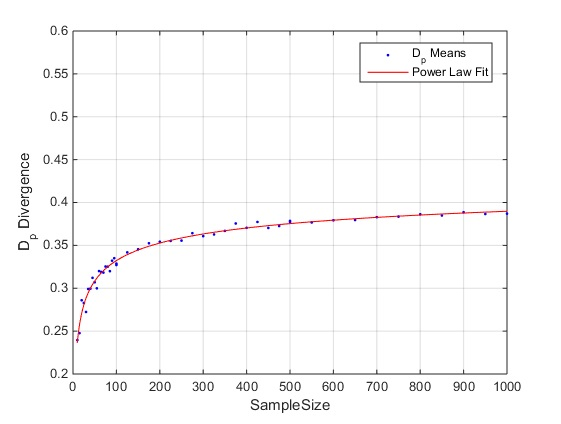
\includegraphics[scale=0.6]{dp_n200_uniform}
		%	\end{center}
	\end{figure}	
	
	\begin{figure}[h!]
		\caption{Distribution of $D_p$ Values for 8-Dimensional Uniform Data Set, N = 200 trials}
		\centering
		%	\begin{center}
		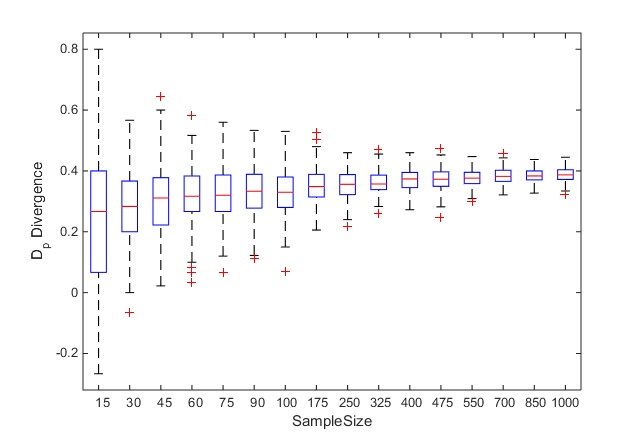
\includegraphics[scale=0.6]{dp_n200_uniform_bars}
		%	\end{center}
	\end{figure}	
\newpage
	\subsection{\small Gaussian Dataset}
	
	
	\begin{table}[!h]
		\caption{Gaussian Dataset for Bootstrap Analysis of $D_p$}
		\centering % used for centering table
		\begin{tabular}{c c c c c c c c c c} % centered columns (4 columns)
			%inserts double horizontal lines
			$D_0$ &  &  &  \\ [0.5ex] % inserts table
			%heading
			\hline % inserts single horizontal line
			$\mu_0$ & 0 & 0 & 0 & 0 & 0 & 0 & 0 & 0\\[0.5ex] % inserting body of the table
			$\sigma_0$ & 1 & 1 & 1 & 1 & 1 & 1 & 1 & 1\\[0.5ex]
			
			$D_1$ & \\ [0.5ex]
			
			\hline
			$\mu_1$ & 0 & 0 & 0 & 0 & 0 & 0 & 0 & 0\\[0.5ex] % inserting body of the table
			$\sigma_1$ & 2.56 & 1 & 1 & 1 & 1 & 1 & 1 & 1\\[0.5ex]
			\hline %inserts single line
		\end{tabular}
		\label{table:nonlin} % is used to refer this table in the text
	\end{table}
	
	\begin{figure}[h!]
		\caption{Asymptotic Convergence of $D_p$ for Gaussian Data Set, N = 50 trials}
		\centering
		%	\begin{center}
		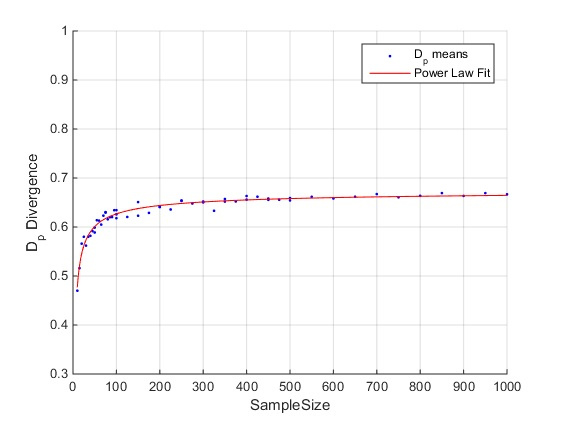
\includegraphics[scale=0.6]{dp_n50_gaussian}
		%	\end{center}
	\end{figure}	
	

	
	\newpage
	\begin{figure}[h!]
		\caption{Convergence of $D_p$ for Banknote Authentication Data Set, N = 50 trials}
		\centering
		%	\begin{center}
		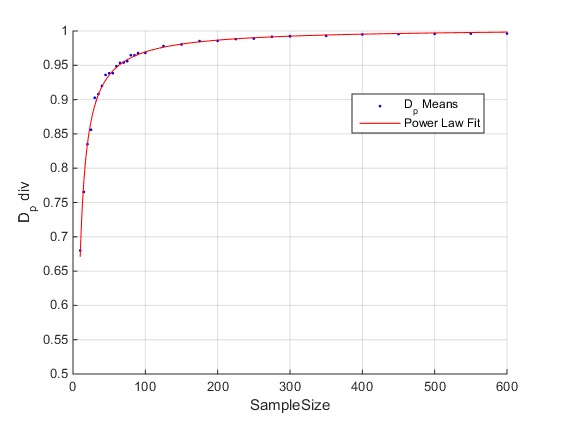
\includegraphics[scale=0.6]{dp_n50_banknote}
		%	\end{center}
	\end{figure}
	
	\newpage
	\subsection{\small Banknote Dataset}
	\indent The empirical example we consider is the Banknote Authentication Data Set taken from the University of California, Irvine Machine Learning Repository [7]. The 4-dimensional dataset contains data extracted from images of banknotes. The data set consists of a relatively small number of dimensions, and highly separated data, so the convergence is rapid, even for relatively small sample size. We note that for a sensitive task such as authenticating banknotes, it should not be surprising to see an asymptotic value for $D_p$ that is close to 1, indicating that the classes are well separated.  
	
	\newpage
	\subsection{\small Pima Indians Dataset}
	
	\begin{figure}[!h]
		\caption{Asymptotic Convergence for Pima Indian Data Set, N = 50 trials}
		\centering
		%	\begin{center}
		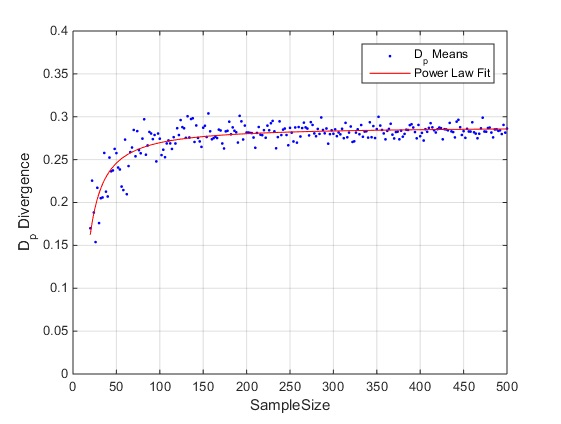
\includegraphics[scale=0.6]{dp_n50_pima}
		%	\end{center}
	\end{figure}
	
	\begin{figure}[!h]
		\caption{Asymptotic Convergence for Pima Indian Data Set, N = 200 trials}
		\centering
		%	\begin{center}
		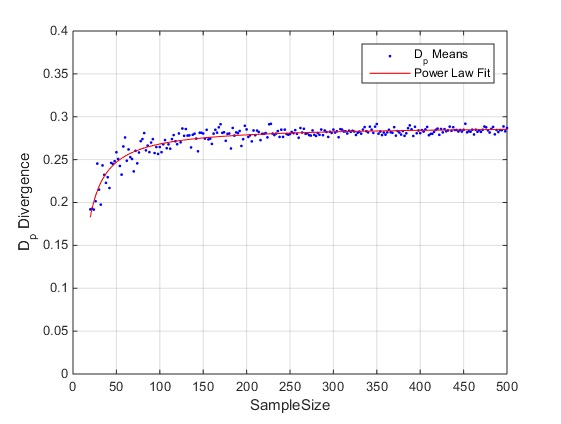
\includegraphics[scale=0.6]{dp_n200_pima}
		%	\end{center}
	\end{figure}	
	
	\begin{figure}[!h]
		\caption{Asymptotic Convergence for Pima Indian Data Set, N = 5000 trials}
		\centering
		%	\begin{center}
		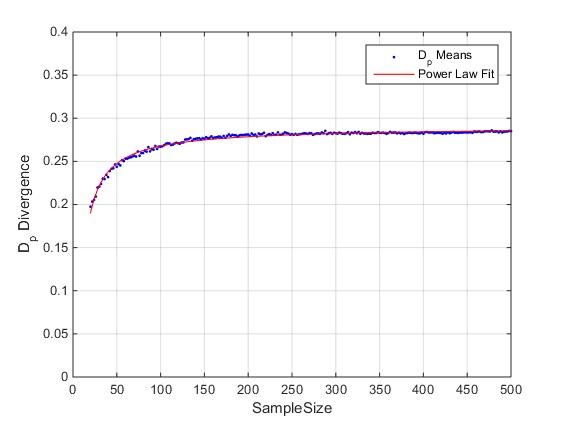
\includegraphics[scale=0.6]{dp_n5000}
		%	\end{center}
	\end{figure}	
	
	%		\begin{figure}[!h]
	%			\caption{Asymptotic Convergence for Pima Indian Data Set, N = 5000 trials}
	%			\centering
	%			%	\begin{center}
	%			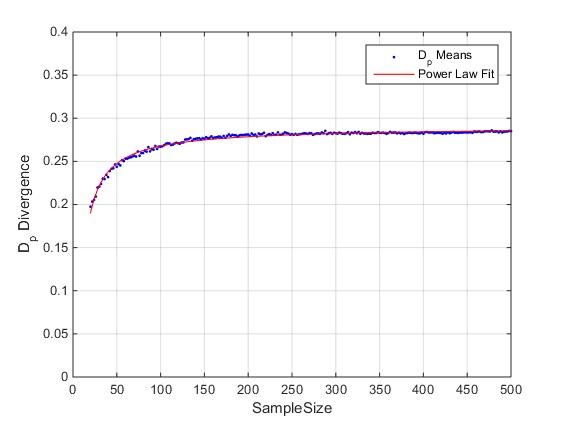
\includegraphics[scale=0.75]{dp_n5000}
	%			%	\end{center}
	%		\end{figure}	
	
	\newpage
	\begin{table}[!h]		
		\caption{Bayes Error Rates in Literature for Pima Indians Data Set [4]}
		\begin{center}
			%	\begin{tabular}{||c c c c||} 
			%		\hline
			\begin{tabular}[!h]{ |p{5cm}||p{4cm}|  }
				
				\hline
				Algorithm & Bayes Error Rate (\%) \\ [0.5ex] 
				\hline\hline
				
				Discrim & 22.50	\\
				Quadisc &  26.20	\\
				Logdisc &  22.30	\\
				SMART  & 23.20	\\
				ALLOC80 &  30.10	\\
				K-NN  & 32.40	\\
				CASTLE &  25.80	\\
				CART  & 25.50	\\
				IndCART &  27.10	\\
				NewID &  28.90	\\
				AC2 &  27.60	\\
				Baytree  & 27.10	\\
				NaiveBay &  26.20	\\
				CN2  & 28.90	\\
				C4.5  & 27.00	\\
				Itrule &  24.50	\\
				Cal5  & 25.00	\\
				Kohonen &  27.30	\\
				DIPOL92 &  22.40	\\
				Backprob  & 24.80	\\
				RBF  & 24.30	\\
				LVQ  & 27.20 	\\ 
				
		%		\textbf{$D_p$}  \\
		%		\textbf{$D_p$ Asymptotic Power Law} & \textbf{22.83} \\ 
				\hline 		
			\end{tabular}
		\end{center}
	\end{table}
	
	
		
	\begin{table}[!h]		
		\caption{Bootstrap Estimated Bayes Error Rates for Pima Indians Data Set [4]}
		\begin{center}
			%	\begin{tabular}{||c c c c||} 
			%		\hline
			\begin{tabular}[!h]{ |p{5cm}||p{4cm}|  }
				\hline
				Algorithm & Bayes Error Rate (\%) \\ [0.5ex] 
				\hline\hline
						$D_p$ (no Bootstrap) & $29.32 \pm 6.22$ * \\
						Efron Bootstrap  & $14.87 \pm 2.465$ ** 	\\
						$m < n$ Bootstrap, $m=200$ & $23.13 \pm 4.13$ 	\\
				\textbf{$D_p$ Asymptotic Power Law} & $\textbf{23.95} \pm \textbf{0.11}$\\ 
				\hline 		
			\end{tabular}
		\end{center}
	\end{table}
	
	\newpage
	\begin{table}[!h]		
		\caption{$D_p$ and Bayes Error Rate for the Pima Indian Data Set for Increasing Sample Size, and Increasing Monte Carlo Iterations}
		\begin{center}
			%	\begin{tabular}{||c c c c||} 
			%		\hline
			\begin{tabular}[!h]{ |p{2cm}||p{2cm}|p{5cm}|p{4cm}|  }
				
				\hline
				Sample Size & Monte Carlo Iterations & $D_p$ Asymptotic Value (95\% Confidence Interval)& Bayes Error Rate (\%), (95\% CI) \\ [0.5ex] 
				\hline\hline
				100	& 50	& 0.2725   (0.245, 0.3)	& $23.90  \pm 1.32$\\
				
				\hline
				
				100	& 200	& 0.2958  (0.265, 0.3267)	& $22.81  \pm 1.42$\\
				\hline
				
				100	& 5000	& 0.3107  (0.2959, 0.3254)	& $22.13  \pm 0.67$\\
				
				\hline
				200	& 50	& 0.2946  (0.2732, 0.3161)	& $22.86  \pm 0.99$\\
				
				\hline 
				200	& 200	& 0.3029  (0.288, 0.3178)	& $22.48  \pm 0.68$\\
				
				\hline
				200	& 5000  & 0.3162  (0.3114, 0.3209)	& $21.88  \pm 0.21$\\
				
				\hline
				300	& 50	& 0.3118  (0.2827, 0.3409)  & $22.08  \pm 1.31$\\
				\hline
				300	& 200	& 0.3073  (0.2926, 0.3219)	& $22.28  \pm 0.66$\\
				\hline
				300	& 5000	& 0.3041  (0.3006, 0.3075)	& $22.43  \pm 0.16$\\ 
				\hline 		
			\end{tabular}
		\end{center}
	\end{table}			
	%	\newpage
	%		\section{Conclusion}
	
%	\Needspace{5\baselineskip}
	\newpage
	\section*{References}[!h]
	[1] Hawes, Chad M., and Carey E. Priebe. "A Bootstrap Interval Estimator for Bayes' Classification Error." 2012 IEEE Statistical Signal Processing Workshop, 2012
	\\ [0.5ex]
	\noindent[2] V. Berisha, A. Wisler, A.O. Hero, and A. Spanias, "Empirically Estimable Classification Bounds Based on a Nonparametric Divergence Measure" IEEE Transactions on Signal Processing, vol. 64, no. 3, pp.580-591, Feb. 2016.
	\\ [0.5ex]
	\noindent[3] A. O. Hero, B. Ma, O. Michel, and J. Gorman, “Alpha-divergence for classification, indexing and retrieval,” Communication and Signal Processing Laboratory, Technical Report CSPL-328, U. Mich, 2001
	\\ [0.5ex]
	\noindent [4] K. Tumer, K. (1996) "Estimating the Bayes error rate through classifier combining" in Proceedings of the 13th International Conference on Pattern Recognition, Volume 2, 695–699
	
	Contains the pima indian dataset BERs in table format
	\\ [0.5ex]
	\noindent[5] Tumer, Kagan, and Joydeep Ghosh. "Bayes Error Rate Estimation Using Classifier Ensembles." International Journal of Smart Engineering System Design 5.2 (2003): 95-109.
	\\ [0.5ex]
	
	\noindent[6] Lichman, M. (2013). UCI Machine Learning Repository [http://archive.ics.uci.edu/ml]. Irvine, CA: University of California, School of Information and Computer Science.
	\\ [0.5ex]
	
	\noindent [7] V. Lohweg, “Banknote Authentication Data Set,” 2012. [Online]. Available: https://archive.ics.uci.edu/ml/datasets/banknote+authentication.
	\\ [0.5ex]
	
	\noindent [8] K. Pranesh, and L. Hunter. "On an Information Divergence Measure and Information Inequalities." (n.d.): n. pag. University of Northern British Columbia. 
	\\ [0.5ex]
	
	\noindent [9] Tukey, J.W. 1958. Bias and confidence in not-quite large samples. Annals of Mathematical Statistics 29: 614
	\\ [0.5ex]
	\noindent [10]Efron, B. "Bootstrap Methods: Another Look at the Jackknife." Annals of Statistics 7.1 (1979)
	\\ [0.5ex]
	
	\noindent [11] https://www.princeton.edu/~verdu/reprints/WanKulVerSep2005.pdf **Create Citation
	\\ [0.5ex]
	\noindent [12] http://www.princeton.edu/~verdu/reprints/WanKulVer.May2009.pdf?q=tilde/verdu/
	reprints/WanKulVer.May2009.pdf **Create Citation
	\\ [0.5ex]
	
	\noindent [13] http://www.eecs.berkeley.edu/~wainwrig/Papers/NguWaiJor10.pdf **Create Citation
	\\ [0.5ex]
	
%	\noindent [14] http://www.stat.yale.edu/~arb4/publications_files/	Distribution Estimation Consistent In Total Variation And In Two Types Of Information Divergence IEEE IT.pdf **Create Citation
%	\\ [0.5ex]

%	\noindent [15] http://www.tsc.uc3m.es/~fernando/bare_conf3.pdf **Create Citation
%	\\ [0.5ex]
	
	\noindent [16] http://arxiv.org/pdf/1404.6230.pdf** Create Citation
	\\ [0.5ex]
	
	\noindent [17] Bootstrap sampling Efron Citation
	\\ [0.5ex]
	
	\noindent [18]
	% http://ac.els-cdn.com/S0019995881902631/1-s2.0-S0019995881902631-main.pdf?_tid=93d74928-deb7-11e5-a4b5-00000aab0f01&acdnat=1456731754_14a794e35c706d6376e880a3eab5c757
	\\ [0.5ex]
	
	\noindent [19]S. Ali and S. D. Silvey, “A general class of coefficients of divergence of one distribution from another,” Journal of the Royal Statistical Society.
	Series B (Methodological), pp. 131–142, 1966.
	%Ali silvey
	\\ [0.5ex]
	
	\noindent [20] Nguyen, Xuanlong, Martin J. Wainwright, and Michael I. Jordan. "Nonparametric Estimation of the Likelihood Ratio and Divergence Functionals." 2007 IEEE International Symposium on Information Theory (2007)
	\\ [0.5ex]

	\noindent [21] Sugiyama, Masashi, Song Liu, Marthinus Christoffel Du Plessis, Masao Yamanaka, Makoto Yamada, Taiji Suzuki, and Takafumi Kanamori. Journal of Computing Science and Engineering 7.2 (2013)
	\\ [0.5ex]
	
	\noindent [22] Nguyen, Xuanlong, Martin J. Wainwright, and Michael I. Jordan. "Estimating Divergence Functionals and the Likelihood Ratio by Convex Risk Minimization." IEEE Trans. Inform. Theory IEEE Transactions on Information Theory 56.11 (2010)
	\\ [0.5ex]
	
	\noindent [23] L. Song, M.D. Reid, A.J. Smola, and R.C. Williamson. Discriminative estimation of f -divergence. Submitted to AISTATS09, October 2008.
	\\ [0.5ex]
	
	\noindent [24] Tumer, Kagan, and Joydeep Ghosh. "Bayes Error Rate Estimation Using Classifier Ensembles." International Journal of Smart Engineering System Design 5.2 (2003)
	\\ [0.5ex]
	
	\noindent [25] Berisha, Visar, and Alfred O. Hero. "Empirical Non-Parametric Estimation of the Fisher Information." IEEE Signal Processing Letters IEEE Signal Process. Lett. 22.7 (2015)
	\\ [0.5ex]
	
	\noindent [26] S. Kullback and R. A. Leibler, “On information and sufficiency,” The	Annals of Mathematical Statistics, pp. 79–86, 1951.
	\\ [0.5ex]
	
	\noindent [27] Wang, Q., S.r. Kulkarni, and S. Verdu. "Divergence Estimation of Continuous Distributions Based on Data-Dependent Partitions." IEEE Trans. Inform. Theory IEEE Transactions on Information Theory 51.9 (2005)
	\\ [0.5ex]
	
	\noindent [28] Wang, Qing, Sanjeev R. Kulkarni, and Sergio Verdu. "Divergence Estimation for Multidimensional Densities Via K-Nearest-Neighbor Distances." IEEE Trans. Inform. Theory IEEE Transactions on Information Theory 55.5 (2009)
	\\ [0.5ex]

	\noindent [29]Barnabás Póczos, Liang Xiong, Jeff G. Schneider, Nonparametric Divergence Estimation with Applications to Machine Learning on Distributions. UAI 2011: 599-608
	
	
\end{document}